% !TEX option = --shell-escape

\documentclass{amsart}


%Preamble
\usepackage{amsmath}
\usepackage{amssymb}
\usepackage{amsthm}
\usepackage{amsrefs}
\usepackage{amsfonts}
%\usepackage{dsfont}
\usepackage{mathrsfs}
\usepackage{mathtools}
%\usepackage{stmaryrd}
%\usepackage[all]{xy}
\usepackage[mathcal]{eucal} % changes meaning of \mathcal
\usepackage{enumerate}
\usepackage[shortlabels]{enumitem}
\usepackage{verbatim} %%includes comment environment
\usepackage{hyperref}
\usepackage[capitalize]{cleveref}
%\usepackage{fullpage} %%smaller margins
\usepackage[all,arc]{xy}
\usepackage{enumerate}
\usepackage{mathrsfs}
\usepackage{graphicx}
\graphicspath{{Images/}}
\usepackage{caption}
\usepackage{subcaption}
\usepackage{setspace}
\usepackage{minted}
\usemintedstyle{colorful}

\hypersetup{
    linktoc=all,     %set to all if you want both sections and subsections linked
}

\newcommand{\bbF}{\mathbb{F}}
\newcommand{\bbN}{\mathbb{N}}
\newcommand{\bbQ}{\mathbb{Q}}
\newcommand{\bbR}{\mathbb{R}}
\newcommand{\bbZ}{\mathbb{Z}}
\newcommand{\bbC}{\mathbb{C}}
\newcommand{\cal}[1]{ \mathcal{#1}}
\newcommand{\Shift}[1]{ \mathcal{S}_{#1}}

\newcommand\restr[2]{{% we make the whole thing an ordinary symbol
  \left.\kern-\nulldelimiterspace % automatically resize the bar with \right
  #1 % the function
  \vphantom{\big|} % pretend it's a little taller at normal size
  \right|_{#2} % this is the delimiter
  }}

\newcommand{\orb}{\mathscr{O}}
\newcommand{\bbCS}{\hat{\bbC}}
\newcommand{\Mand}{\cal{M}}

\newcommand{\PSL}{\operatorname{\textbf{PSL}}}
\newcommand{\Poly}{\operatorname{Poly}}
\newcommand{\NW}{\operatorname{NW}}

\newcommand{\abs}[1]{ \left| #1 \right| }
\renewcommand{\phi}{\varphi}
\renewcommand{\emptyset}{\O}

%--------Theorem Environments--------
%theoremstyle{plain} --- default
\newtheorem{thm}{Theorem}[section]
\newtheorem{cor}[thm]{Corollary}
\newtheorem{prop}[thm]{Proposition}
\newtheorem{lem}[thm]{Lemma}
\newtheorem{conj}[thm]{Conjecture}
\newtheorem{quest}[thm]{Question}

\theoremstyle{definition}
\newtheorem{defn}[thm]{Definition}
\newtheorem{defns}[thm]{Definitions}
\newtheorem{con}[thm]{Construction}
\newtheorem{exmp}[thm]{Example}
\newtheorem{exmps}[thm]{Examples}
\newtheorem{notn}[thm]{Notation}
\newtheorem{notns}[thm]{Notations}
\newtheorem{addm}[thm]{Addendum}
\newtheorem{exer}[thm]{Exercise}

\theoremstyle{remark}
\newtheorem{rem}[thm]{Remark}
\newtheorem{obs}[thm]{Observation}
\newtheorem{rems}[thm]{Remarks}
\newtheorem{warn}[thm]{Warning}
\newtheorem{sch}[thm]{Scholium}

\makeatletter
\let\c@equation\c@thm
\makeatother
\numberwithin{equation}{section}
\bibliographystyle{abbrv}

\title{Complex Dynamics \& Computation}\author{Marlin Figgins}
\date{March 21, 2019\\ Last Updated: \today}



\begin{document}
	\maketitle

\tableofcontents

	\section*{Introduction}

%This will be my introduction paragraph and will discuss why I decided to do complex dynamics and computation! Providing a small tour of attractions and hopefully highlighting the relation between the things I picked to discuss. Note: I'm going to be writing all the code discussed in this paper, so I'm also going to present code snippets to highlight the interplay between the theory and the computation, but because of that I'm going to be skipped the implementation of most of the visualization stuff because there's not much relation to the actual mathematics there.\\

Complex dynamics is fundamentally the study of iterated holomorphic functions. Given a holomorphic function $f:\bbCS\to \bbCS$, we want to analyze the behavior of its iterates. For a given $n\in\bbN$, we define the $n$-th iterate of $f$ as
\[
f^n=\underbrace{f\circ f\circ \dotsb \circ f}_{n \text{ times}}.
\]
Primarily, we will study the orbit of a point $z\in\bbC$ under $f$, $\orb(f,z)=\orb(z)=\{f^n(z)\mid n\in \bbN_0 \}$. The general goal of this being to understand the dynamics of $f$ i.e. its fixed and periodic points, where points tend to under iteration, and the sensitivity of the orbits of $f$ to different initial conditions. In particular, we will take advantage of the continuity of $f$ and the compactness of $\bbCS$ and many of our questions will pertain to the sensitivity of $f$ to initial conditions and the recurrence of orbits, which immediately remind of the wandering and non-wandering sets. In this way, it is clear that, to some extent, we want to be able decompose our space $\bbCS$ according to the dynamics $f$. For the purposes of this paper, we will mainly restrict our attention to the iteration of rational functions of the Riemann sphere.\\

Complex dynamics as a field gained new life by early attempts to visualize the Mandelbrot set which we will define and discuss at length later. This sparked an increased use of computation and attempts to visualize some of the natural and recurrent objects in complex dynamics. Using these methods, the natural visual beauty of complex dynamics becomes even more apparent and thrilling! Some may say that it is one thing to theorize and another to compute, but complex dynamics is a clear example in which both of these coexist and inform one another to fully highlight the various complexities and simplicities of the subject. In this paper, we will attempt to highlight the interplay of visualization, computation, and theory. Starting with the classical example of M\"{o}bius transformations and rational maps on the Riemann sphere $\bbCS$ and moving onto the study of polynomials in degree two and three, we will analyze and present some of the methods and algorithms used to model and visualize complex dynamical systems as well as the theory motivating them!

  %This will be my final paper and I'm very stressed about it! The main point of this paper will to be to provide a light introduction to complex dynamics and to explore computation (and the underlying theory making it possible) as a tool to help visualize and inform our understanding of complex dynamics! This includes visualizing Julia sets and Mandelbrot sets and understanding several different algorithms that can be used in their computation! We will start with dynamics of Möbius transformations on the Riemann Sphere (possibly visualizing and computing them)


  %%Possibly explore limit sets of rational maps, discuss domain covering


   %and then proceed to the study degree two polynomials, focusing on the theory behind the algorithms used to compute their Julia Sets and the famous Mandelbrot set. We will finally discuss the application of these methods to the problem of computing and visualizing the Shift Locus.

%%% Ultimately our interest is on the iteration of holomorphic functions, but an important aspect of this is the visualization of these functions and their iterations as a complement to our theoretical understanding of their behavior. Therefore, I will start with methods used to visualize the complex plane

%\section{Visualization of the Complex Plane}

%Having a struggle to figure out if this section is necessary given what will come later!

%\subsection{Importance of Visualization}
%This will probably be a paragraph about how visualization can a quick way of presenting qualitative information, provide intuition to a problem.

%Different methods of visualization can make it easy to identify

%\subsection{Domain Coloring}
%\begin{itemize}
%  \item Basic ideas behind domain covering i.e. coloring functions and HSV space. Using it to identify poles, zeroes, etc.
%\end{itemize}

%subsection{Visualizing Riemann Surfaces}
%This section will probably be hard to finish the code for, so I'm probably going to have to cite someone else's and modify it to deal with the last case.

  %\begin{itemize}
  %\item Multi-valued functions and visualizing them focusing on $\sqrt{z}$.
  %\item Mention relation to $z^2+c$ and Danny's `pants' example.
%\end{itemize}
  %% Double Branch Covers ... \sqrt{z}

%%% In particular, we may want to visualize the Riemann sphere and actions on it...

\section{Basic Complex Dynamics}

Shifting our focus to complex dynamics, we will define some notions that will be of interest in the sections to come. Many of the fundamental questions in complex dynamics concern the qualitative behavior of orbits such as whether they are periodic, dense in some set, attracted to or repelled from a point.

The first object we will concern ourselves with is the non-wandering set.

\begin{defn}
  Given a holomorphic function $f$, the \emph{non-wandering set of $f$} $\NW(f)$ is the set of points for which every open set $U$, there exists a positive integer $n$ such that \[
f^n(U)\cap U\neq\emptyset
  \]
\end{defn}
The non-wandering set of $f$ is closed, $f$-invariant. This means that each neighborhood $\bbCS$ eventually returns to itelf under the dynamics of $f$. This is contrasted with the wandering set, the set of points for which there is a neighborhood that never returns to itself. Since the wandering set is the complement of the non-wandering set, these two sets are provide a classification the general behavior of points since $\bbCS$ can be written as a disjoint union of these two sets.\\

As we will see through results such as the No-Wandering-Domain theorem (\cref{NWDT}), these sets do not completely describe the kinds of behaviors we're interested in the case of complex dynamics and we will develop the ideas of the Julia and Fatou sets to deal with some of the particularities of the complex case.

%%%%%Mention NO WANDERING DOMAIN THEOREM

To begin studying these behaviors, we're going to need to develop an understanding of the \emph{fixed points of $f$} i.e. points $z$ such that $f(z)=z$.

\begin{defn}\label{multiplier}
Given a holomorphic function $f$ and fixed point $z_0$, we define the \emph{multiplier of $f$ at $z_0$} to be $\abs{f'(z_0)}$. Moreover, we call $z_0$
\begin{enumerate}
  \item \emph{super-attracting} if $\abs{f'(z_0)}=0$,
  \item \emph{attracting} if $0<\abs{f'(z_0)}<1$,
  \item \emph{indifferent} if $\abs{f'(z_0)}=1$,
  \item \emph{repelling} if $\abs{f'(z_0)}>1$.
\end{enumerate}
\end{defn}

The multiplier of a fixed point can provide important information about the dynamics near a point. As we will see, this multiplier is an invariant under conformal conjugacies. Much of studying dynamical systems is concerned with those properties that are preserved under conjugacy. In the case of complex dynamics, we are interested in systems that conformally conjugate and those invariants.

\begin{defn}
  We say that holomorphic maps $f$ and $g$ are \emph{conformally conjugate} if there is some biholomorphic map $\phi$ such that
  \begin{equation}
    f\circ \phi =\phi \circ g.
  \end{equation}
\end{defn}
\begin{rem}
  Henceforth, all conjugacies are assumed to be conformal conjugacies unless stated otherwise.
\end{rem}
Periodic orbits (including fixed points) are preserved under conjugacy as well as other dynamical properties such as transitivity, mixing, and entropy. Therefore, we can consider it to be a sort of `change of coordinates.' In particular, we can see that $\phi$ additionally preserves multipliers.
\begin{prop}
  If $f$ and $g$ are conjugate and $z_0$ is a fixed point of $f$, then $z_0$ and $\phi(z_0)$ have the same multiplier.
\end{prop}
\begin{proof}
  This is an application of the chain rule for holomorphic functions paired with the definition of conjugacy.
\end{proof}
In the following section, we'll apply these ideas to classify the dynamics of degree one rational functions on the Riemann Sphere.

\subsection{M\"{o}bius Transformations \& the Riemann Sphere}
  We begin by analyzing the M\"{o}bius transformations which are the conformal automorphisms of the Riemann Sphere. %%% Ugly Sentence...

  \begin{defn}
    A \emph{M\"{o}bius Transformation} is a map $f\colon
  \bbCS\to\bbCS$ of the form
    \begin{equation}
      f(z)=\frac{az+b}{cz+d},
    \end{equation}
    where $a,b,c,d\in\bbC$ and $ad-bc\neq 0$.
  \end{defn}
  \begin{rem}
  When dealing with M\"obius transformations, we adopt the following rules so that $f$ is properly an automorphism of the Riemann sphere:
  \begin{enumerate}
    \item If $c\neq 0$, $f(-\frac{d}{c})=\infty$  and $f(\infty)=\frac{a}{c}$.
    \item If $c=0$, $f$ is linear map and we define $f(\infty)=\infty$.
  \end{enumerate}
  \end{rem}


For any given $\lambda\neq 0$, the M\"obius transformation defined by the coefficients $\lambda a, \lambda b, \lambda c, \lambda d$ is the same as the one described by $a,b,c,d$ i.e.
  \[
f(z)=\frac{(\lambda a )z+(\lambda b)}{(\lambda c)z+(\lambda d)}=\frac{az+b}{cz+d}.
  \]
Therefore, we can always normalize, so that $ad-bc=1$. We will only consider such M\"obius transformation in what follows. In doing this, we can relate the set of M\"obius transformations with the group of matrices
\[
\PSL(2,\bbC)=\left\{  \begin{pmatrix}
a & b\\
c & d
\end{pmatrix} \,\middle\vert\, ad-bc=1 \text{ where $a,b,c,d\in\bbC$}\right\}.
\]
In fact, a quick computation shows that this set of normalized M\"obius transformations (under composition) is isomorphic to $\PSL(2,\bbC)$ (under matrix multiplication) as a group. This observation is simple, yet powerful in our study of the M\"obius transformations and their dynamics.

\begin{obs}
The composition of M\"obius Transformation is again a M\"obius transformation.
\end{obs}

This observation helps to elucidate our problem. If we're interested in understanding the dynamics of a particular M\"obius transformation on the Riemann Sphere, it is essential to understand the group of M\"obius transformations themselves. Therefore, we begin by an analysis of the fixed points of a given M\"obius transformation.

\begin{lem}
  Every non-identity M\"obius transformation $f(z)=\frac{az+b}{cz+d}$ has one or two fixed points.
\end{lem}

\begin{proof}
  In the case $c=0$, we can reduce to the linear equation $f(z)=az+b$. Clearly, $f$ fixes $\infty$, so we're left to check whether $z=az+b$ has a solution. If $a=1$, then there is no solution. Otherwise, $\frac{b}{1-a}$ is a solution. This means $f$ has at most 2 solutions.

Otherwise $c\neq 0$. We can attempt to solve for the fixed points directly and see that the equation
\[
f(z)=\frac{az+b}{cz+d}=z
\]
can be rewritten as the equation for the roots of a quadratic polynomial
\[
cz^2+(d-a)z-b=0,
 \]
 which must have two solutions (counting multiplicity) by the Fundamental Theorem of Algebra.

\end{proof}

Using the quotient rule, we can compute the derivative of a M\"obius transformation $f$ as
\begin{equation}
  f'(z)=\frac{ad-bc}{(cz+d)^2}.
\end{equation}

Our knowledge about the derivative at a fixed point gives us information about the orbits of our dynamical system.  In the case of M\"obius transformations, the fixed points and their multipliers allow us to completely classify their dynamics.

\begin{thm}
  Let $f$ be a non-constant M\"obius transformation. Then if $f$ has single fixed point $z_0$, every orbit of $f$ coverages to it. Otherwise, $f$ has two fixed points $z_1, z_2$  and one of the following holds:
  \begin{enumerate}
    \item every orbit of $f$ converges to one of the fixed points,
    \item every orbit is finite,
    \item or forms a dense subset of some circle.
  \end{enumerate}

\end{thm}

\begin{proof}
Suppose $f$ has exactly one fixed point at $\infty$. Then we can write $f(z)=z+b$ where $b\neq0$. We see that $f^n(z)=z+nb$ and that every orbit must go off to infinity. If $f$ has a fixed point $z_0$, then we can conjugate using $\phi(z)=\frac{1}{z-z_0}$ to see that
\[
g(z)=\phi\circ f\circ\phi^{-1}(z)
\]
must fix $\infty$. Therefore, every orbit of $g$ goes off to $\infty$. This tells us that the orbit of $f=\phi^{-1}\circ g\circ \phi$ must approach $\phi^{-1}(\infty)=z_0$.\\

If $f$ instead has two fixed points, let them be at $0$ and $\infty$. Therefore, we can write $f(z)=\lambda z$. This leaves us three possibilities for the parameter $\lambda$, $\abs{\lambda}<1, \abs{\lambda}>1, \abs{\lambda}=1$. If $\abs{\lambda}<1$, then $f^n(z)$ goes to 0 as $n$ goes to infinity. Similarly, if $\abs{\lambda}>1$ the orbit of $f$ goes to $\infty$. If $\abs{\lambda}=1$, then $\lambda$ is either a root of unity or not. In the former case, there is some $n$ such that $f^n(z)=\lambda^n z=z$. In the latter, $f(z)$ acts like an irrational rotation of the circle of radius $\abs{z}$ and therefore, its orbit is dense on that circle.

Similar to before, if $f$ has distinct fixed points $z_1$ and $z_2$, we can find a M\"obius transformation $\phi$ that maps $z_1$ to 0 and $z_2$ to $\infty$ for example, $\phi(z)=\frac{z-z_1}{z-z_2}$. This finishes the proof since $g=\phi\circ f\circ\phi^{-1}$ fixes 0 and $\infty$.
 \end{proof}

 This theorem completely classifies the dynamics of rational maps of degree one by conjugating any M\"obius Transformation to the map $z\mapsto z+b$ or $z\mapsto \lambda z$.  As one might expect, we will find that the dynamics of higher order rational functions will not behave as nicely. Because of this, visualization may become an increasing useful aid in getting an intuition for the more complicated dynamics of higher degree rational maps.

  \begin{defn}
    A \emph{rational function} is a function $f:\bbCS\to\bbCS$ of the form
    \begin{equation}
      f(z)=\frac{P(z)}{Q(z)}=\frac{a_nz^n+\dotsb+ a_0}{b_mz^m+\dotsb+ b_0},
    \end{equation}
    where the numerator $P(z)$ and denominator $Q(z)$ are polynomials with complex coefficients and not both identically zero.
  \end{defn}
  \begin{rem}
    If the polynomials $P$ and $Q$ above are co-prime, we define the degree of $f$ to be maximum of the degrees of $P$ and $Q$ as polynomials i.e. $\max(n,m).$
\end{rem}

Degree is a helpful notion that we can use to describe the `complexity' of a function or, loosely, the number of different paths or branches one can take to arrive at a given point.

  \begin{prop}
    If $f$ is a non-constant rational function of degree $d>0$, then $f$ is a $d$-fold map from $\bbCS$. That is, every point $z\in\bbCS$ has exactly $d$ pre-images.
  \end{prop}

  %%% Make note about degree of polynomial to itself. Every $w$ has $d$ pre-images. Include proof which is kinda on 31.

If we note that the degree of rational maps multiply under composition, we can derive the following corollary about the iterates of rational maps.

\begin{cor}\label{ExpDeg}
  If $f$ is a rational map of degree $d$, then $f^n$ is a rational map of degree $d^n$.
\end{cor}
This corollary suggests that the number of periodic points of period $n$ grows exponentially in $n$ since the rational function $f^n(z)-z$ has the same degree as $f^n$, meaning that the behavior of $f^n$ is increasingly complicated and exponentially so.

With an understanding of the most basic types of holomorphic dynamical systems, we can begin to define some of the central objects of complex dynamics.

\subsection{The Fatou and Julia Sets}

The Julia and Fatou sets give us a way of splitting the dynamics of a map $f$ into a set of `niceness' on which the dynamics of $f$ are locally tame and a set of `chaos' on which dynamics are sensitive to initial conditions. Heuristically, we will call the Fatou set the set of points on which the iterates of $f$ are locally well behaved and the Julia set its complement. In order to make this notion rigorous, we rely on the notion of normality as introduced by Paul Montel (1912). %%% introduced by Montel Blah Blah Blah.

\begin{defn}
A family of functions $\cal{F}$ on $X$ is called \emph{normal} if every sequence of functions in $\cal{F}$ has a subsequence $f_n$ that converges to a function $f$ locally uniformly. That is, every point $z\in X$ has a neighborhood $U$ on which  $\restr{f_n}{U}$ converges to $\restr{f}{U}$.
\end{defn}

This gives us a notion of how a family of functions can be well behaved. From the point of view of dynamics, the family of functions we're interested in is the collection of iterates of $f$.

\begin{defn}
  Given a non-constant rational function $f$ on the Riemann Sphere, the \emph{Fatou set} $F(f)$ is the domain on which the family $\{f^n\mid n\in\bbN\}$ is normal. We define \emph{Julia set} $J(f)$ to be the complement of the Fatou set.
\end{defn}

From this definition, it is clear that $F(f)$ is open and that $J(f)$ is closed. Likewise, it follows that points on the Julia set are \emph{sensitive to initial conditions} in the following sense. Any neighborhood of a point in $J(f)$ must contain points exhibiting distinct dynamical behaviors. We will see an example of this later when we discuss the dynamics of the map $z\mapsto z^2$.\\

Another useful lemma for understanding the structure of Julia sets is the fact that it is invariant under the map $f$.

\begin{lem}\cite[Lemma 4.4]{milnor2011}
  The Julia set $J(f)$ of any holomorphic function $f$ is fully invariant i.e. $f^{-1}(J(f))=J(f)=f(J(f))$.
\end{lem}

With this knowledge, it is clear that the Julia and Fatou sets give an $f$-invariant decomposition of $\bbCS$ into two sets of points, one of which is sensitive to initial conditions and another which exhibits `tame' local dynamics under $f$.

With this in mind, we can also relate the Julia set with the non-wandering set which was our prototype for dealing with the type of recurrence and sensitivity expected by the Julia set.

When dealing with polynomials, we will often try to compute the filled Julia set of a map $f$ instead of just its Julia sets.

\begin{defn} If $f$ is a monic polynomial. the \emph{filled Jula set $K(f)$} is the set of points $z$ for which the orbit $\orb(f)$ is bounded.
\end{defn}

This will be useful in the sense that the filled Julia set $K(f)$ is precisely the complement of the basin of attraction to $\infty$ for a given monic polynomial $f$.

Returning the idea of the non-wandering set discussed earlier, we can derive the following relationship between the Julia set and the non-wandering set.

\begin{prop}
  The Julia set $J(f)$ is contained in the $\NW(f)$.
\end{prop}

It turns out that the reverse inclusion might not hold, the two sets are not necessarily equal. The picture is a bit more complicated as Problem 19-A of Milnor \cite{milnor2011} shows.

\begin{thm}\cite[Problem 19-A]{milnor2011}
For a rational function $f\colon \bbCS\to \bbCS$, the non-wandering set $\NW(f)$ is the disjoint union of its Julia set, its attracting periodic points, and rotation domains.
\end{thm}

This tells us that the non-wandering set is a useful aid in our intuition and understanding the dynamics of $f$ and the Julia set, but does not characterize it entirely.

A similar statement for the Fatou set was proved by Dennis Sullivan in 1985.
\begin{thm}[No-Wandering-Domain Theorem]\cite{sullivan1985quasiconformal}\label{NWDT}
  Any rational map $f\colon\bbCS\to\bbCS$ of degree greater than two has no wandering domain.
\end{thm}

This leads us to study the Julia and Fatou sets as separate entities entirely, which better characterize our ideas of `locally' tame dynamics. As of now, we have defined and worked with some of the properties of the Julia set, but some natural questions are `what do the dynamics on the Julia set actually look like?' and `what is the the actual form of the Julia set?'. To approach these questions, we're going to rely on some computational methods.

  \subsection{Computing the Julia Set}\label{JuliaComp}

Knowing the shape of a given holomorphic function's (filled) Julia set can help gain insight into a given functions dynamics. In the case of polynomials, the filled-in Julia set gives us a way of distinguishing points whose orbits remain bounded, localizing their dynamics. Knowing the actual shape of this set as well as its different connected components gives us an idea of how bounded orbits of points may permute or move between the components of the Fatou set.

\begin{cor}\cite[Corollary 4.13]{milnor2011}
For any given $z$ in the Julia set $J(f)$,
\[
\bigcup_{n=1}^{\infty}f^{-n}\{z\}
\]is dense in $J(f)$
\end{cor}

Simply computing the Julia set by taking pre-images of a specific point is na\"ive in the sense that for any non-constant rational map $f$ of degree $d$ taking $n$ pre-images of a point $z$ leaves you to compute $d^n=\abs{f^{-n}\{z\}}$ points of your Julia set. For example, if $f$ is only of degree 2, after taking only 40 pre-images you're left to compute more than a trillion points! This further becomes an issue because there is no promise of how many iterates it will take to get close to any particular point in $J(f)$. Though there are methods adapting this idea to make it more computationally efficient, we will explore a differnt route for computing the Julia set.

Another way to do this may be to track whether or not a given orbit of a point diverges to $\infty$ under a rational map $f$. For computational efficiency, we will instead check if the orbit escapes some bailout (or escape) radius $b$ and find the number of iterates it takes for a given point to escape. In Python, we can implement this process as follows:

\inputminted[mathescape]{python}{code-snippets/Julia.py}

We can then apply this function to a range of pixels using the following code snippet and generate an image of the Julia set in a particular region of the plane.

\inputminted[mathescape]{python}{code-snippets/Julia_Set.py}

This algorithm allows us to produce pictures of the Julia set for any given complex function $f$. Examples of such pictures are shown in \cref{fig:JuliaSets}.

\begin{figure}[h]
\centering
\begin{subfigure}{.32\textwidth}
  \centering
  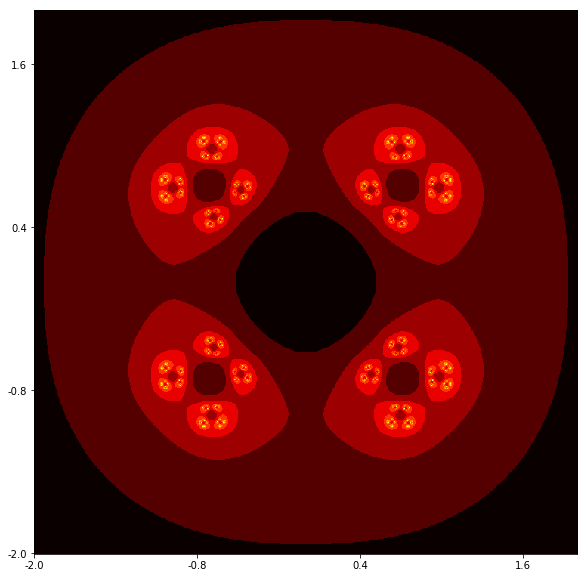
\includegraphics[width=.8\linewidth]{Juliaz2pluszneg2.png}
  \caption{$z\mapsto z^2+\frac{1}{z^2}$}
\end{subfigure}%
\begin{subfigure}{.32\textwidth}
  \centering
  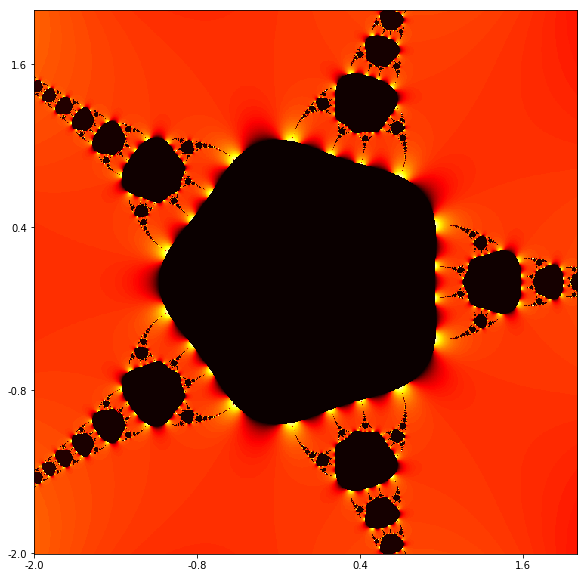
\includegraphics[width=.8\linewidth]{Juliaz5-4dividez4.png}
  \caption{$z\mapsto \frac{z^5-4}{z^4}$}
\end{subfigure}
\begin{subfigure}{.32\textwidth}
  \centering
  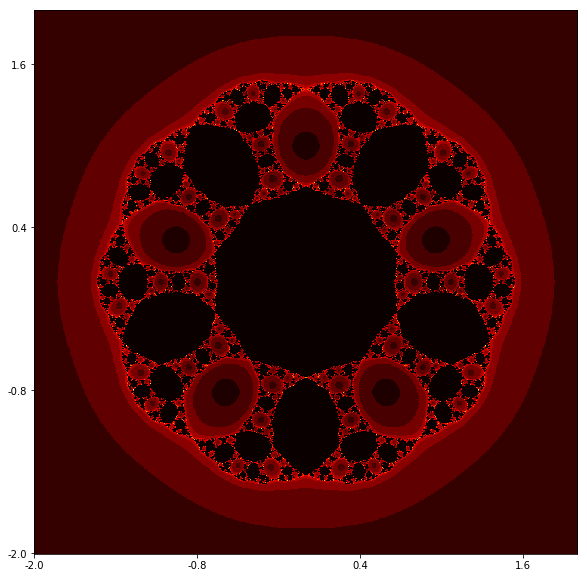
\includegraphics[width=.8\linewidth]{JuliaFunky2.png}
  \caption{$z\mapsto \frac{iz^5-1}{z^5-i}$}
\end{subfigure}
\begin{subfigure}{.32\textwidth}
  \centering
  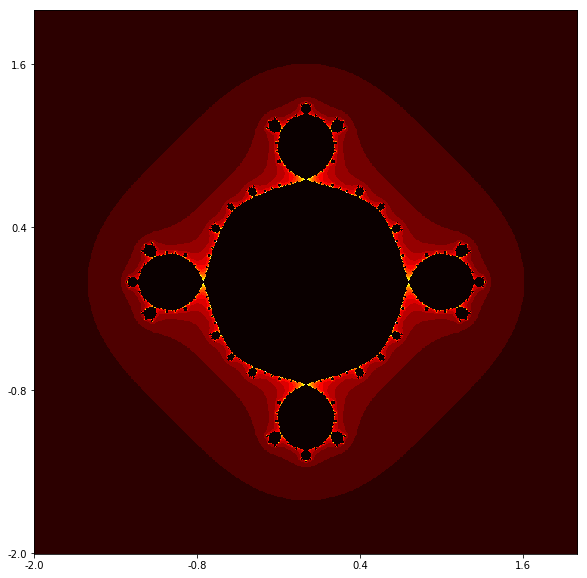
\includegraphics[width=.8\linewidth]{Julia075z4minus1.png}
  \caption{$z\mapsto \frac{3}{4}z^4-1$}
\end{subfigure}
\begin{subfigure}{.32\textwidth}
  \centering
  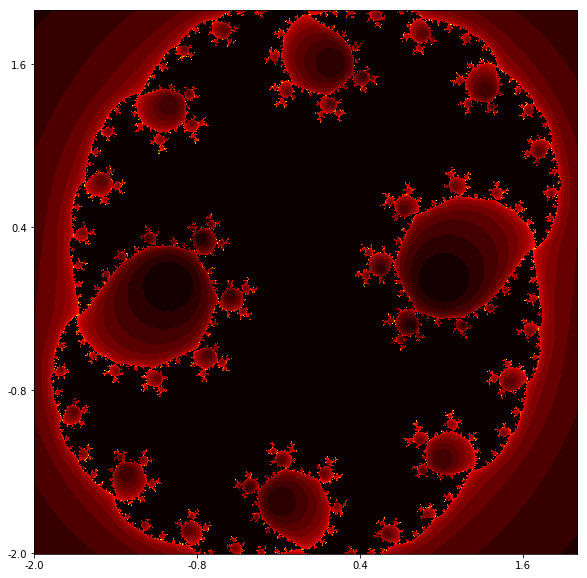
\includegraphics[width=.8\linewidth]{JuliaFunky.png}
  \caption{$z\mapsto \frac{z^2+i}{1-z^2}$}
\end{subfigure}
\caption{Example Julia sets computed with above code.}
\label{fig:JuliaSets}
\end{figure}

As one can see, these Julia sets can be quite complicated. This is reflected by the run time of our code which takes on average 5.95 seconds $\pm$ 331 milliseconds\footnote{All timing benchmarks in this paper are taken as a time average of 7 runs and computed using a $720\times 720$ grid of pixels and a maximum of 500 iterates.} to generate the figures like those in \cref{fig:JuliaSets}. One main cause of this being that the julia function above takes an arbitrary function $f$ as argument which, then, must be applied repeatedly. This can lead to quite a bit of slow-down which we can alleviate by hard coding in the function we'd like to iterate with. In particular, we can replace the julia function from the code snippets above to adapt it to compute the Julia sets for the family of functions of the form $f_c(z)=z^2+c$ where $c$ is any complex number. We will discuss this dynamics of this family in more detail in later sections of this paper, but for now, we can use our above Julia function with the following edits to compute the Julia sets for members of this family:
\inputminted[mathescape]{python}{code-snippets/Juliaquad.py}

Examples of these Julia sets can be seen in \cref{fig:JuliaSetsC}. The decision to take in the complex value $c$ as an argument instead of an arbitrary function $f$ leads to significant speed-up in computation, each run taking 29.1 milliseconds $\pm$ 763 microseconds on average.

\begin{figure}[h]
\centering
\begin{subfigure}{.32\textwidth}
  \centering
  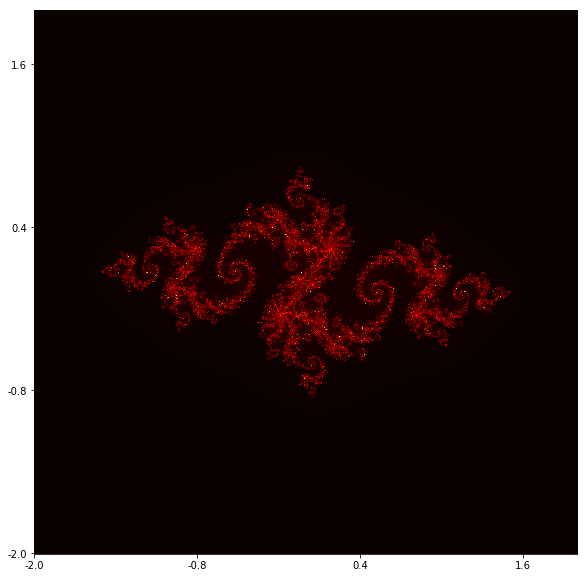
\includegraphics[width=.8\linewidth]{JuliaC1.png}
  \caption{$c=-0.79+0.15i$}
\end{subfigure}%
\begin{subfigure}{.32\textwidth}
  \centering
  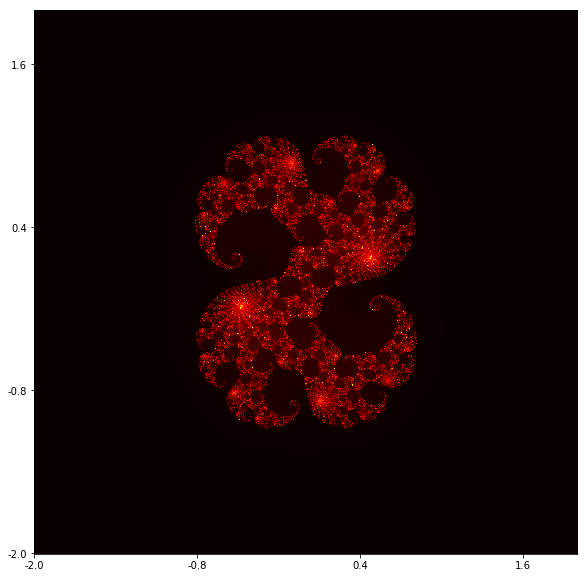
\includegraphics[width=.8\linewidth]{JuliaC2.png}
  \caption{$c=0.28+0.009i$}
\end{subfigure}
\begin{subfigure}{.32\textwidth}
  \centering
  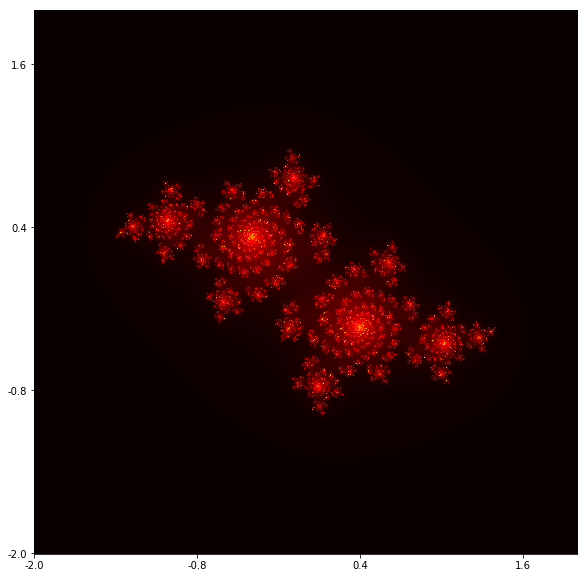
\includegraphics[width=.8\linewidth]{JuliaC3.png}
  \caption{$c=-0.44+0.59i$}
\end{subfigure}
\begin{subfigure}{.32\textwidth}
  \centering
  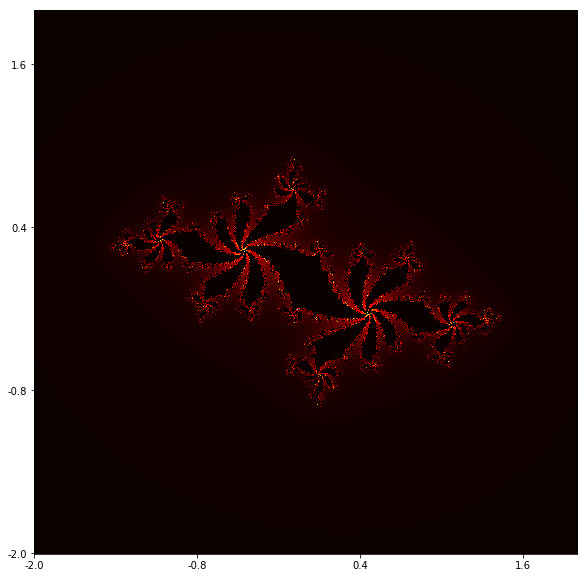
\includegraphics[width=.8\linewidth]{JuliaC4.png}
  \caption{$c=-0.62+0.437i$}
\end{subfigure}
\begin{subfigure}{.32\textwidth}
  \centering
  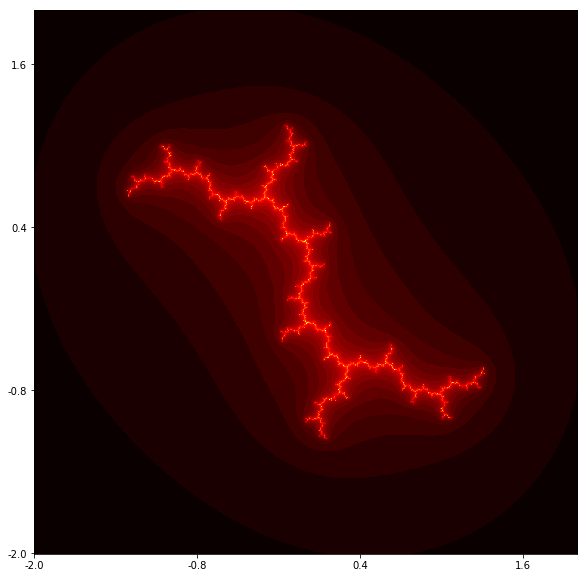
\includegraphics[width=.8\linewidth]{JuliaCi.png}
  \caption{$c=i$}
\end{subfigure}
\caption{Examples of Julia sets of $f_c(z)=z^2+c$ for certain $c$ values.}
\label{fig:JuliaSetsC}
\end{figure}

We can see there's a variety of structures in the Julia sets produced by this algorithm. Most of them seem to be fractal-like. Some are connected while others appear to be specks of what looks like `dust', we will see later that connectedness of the Julia set is related to the Mandelbrot set. We will see these kinds of connections as we shift our study to the polynomials and later, the family of polynomials $f_c(z)=z^2+c$ in the next sections.

\section{Iterating Polynomials}

We will begin our study of iterated complex polynomials with the most simple case of degree two polynomials. For simplicity's sake, we will start by studying $z\mapsto z^2$.

\subsection{The case of $z\mapsto z^2+c$}

Consider the squaring map $f\colon z\mapsto z^2$. For this map given any $n\in\bbN$, we can write an explicit formula for the $n$-th iterate of $f$ \[
f^n(z)=z^{2n}.
\]
Using this formula, we can easily deduce the dynamics of $f$ off the unit circle.
\begin{prop}
Under $f(z)=z^2$, every point that is not on the unit circle is attracted to either 0 or infinity. Moreover, the Julia set $J(f)$ is the unit circle $S^1=\{z\mid \abs{z}=1\}$.
\end{prop}

\begin{figure}[h]
\centering
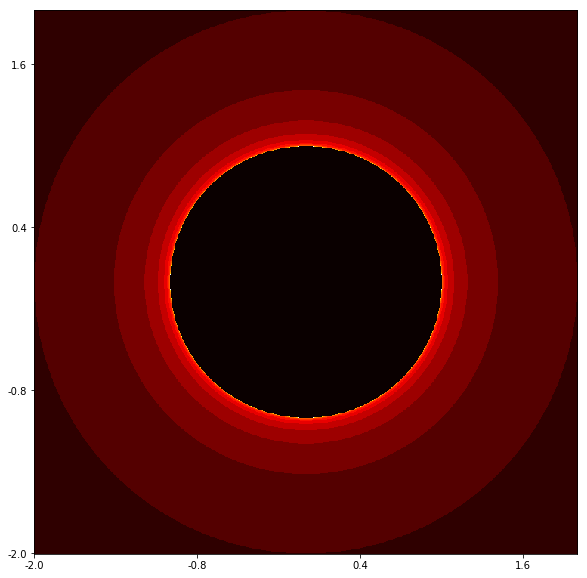
\includegraphics[width=0.33\linewidth]{Juliaz2.png}
\caption{The filled Julia set of $z\mapsto z^2$.}

\end{figure}

%%%%%%% Enter Picture of Julia Set for $z^2$
The dynamics on the Julia set $S^1$ of $z\mapsto z^2$ can be related to a familiar and well-studied dynamical system. We can present each point $z$ of $S^1$ uniquely as $e^{2\pi i \theta}$ for some $\theta\in[0,2\pi)$. We can see that $z\mapsto z^2$ acts as $e^{2\pi i \theta}\mapsto e^{2\pi i (2\theta)}$ in $S^1$. This is clearly the doubling map on $S^1=\bbR/\bbZ$ which we know to be sensitive to initial conditions. We can see that $S^1$ serves as the boundary for two different dynamics behaviors. Any neighborhood of a point on $S^1$ contains a connected component inside the unit circle which is attracted to $0$ and another outside the unit circle which is attracted to $\infty$. This tell us that the filled Julia set $K(f)$ is precisely the closed unit disk $\overline{\mathbb{D}}=\{z\mid \abs{z}\leq 0\}$.
  %%%Julia Set is a circle, what happens on this?


Since we're interested in studying other degree two polynomials, we will shift our attention to the family of polynomials $f_c(z)=z^2+c$ where $c$ is any complex number. Unlike the case where $c=0$, the dynamics of $f_c$ are often not as simple and the Julia sets not as easily understood. Different values of $c$ can cause $f_c$ to have drastically different dynamics. To see this consider $c=-1,1, i $, we can write the orbits of 0 under each $f_c$ as sequences $(z_n)_{n=1}^\infty=f^n_c(0)$:
\begin{align}
   (z_n)&=-1, 0 , -1, 0, \ldots \text{\ \ when $c=-1$}, \\
    (z_n)&=1, 2, 5, 26, 677 \ldots\text{ when $c=1$}, \\
  (z_n)&=i, -1+i, -2i, \ldots \text{ when $c=i$}.
\end{align}

From this, we can see that various types of behavior are possible for different values of $c$. More generally one might ask what are all of the possible behaviors for the sequences $(z_n)_{n=1}^\infty$ defined by \[
0, z_1=f_c(0), z_2=f(z_1), z_3=f(z_2), \ldots
\] Another aspect of this question is asking what happens to our family of functions $\cal{F}_c=\{f_c\mid c\in\bbC\}$ as we move through the parameter space of $c$ \emph{continuously}. Already, we can get some elementary estimates of the behavior of $z\mapsto z^2+c$ outside a neighborhood of 0.

\begin{prop}[Bailout Radius for $z\mapsto z^2+c$]\label{Mescape}
  For any $c\in\bbC$, if the $f_c$-orbit of 0 escapes the circle of radius 2, then it goes off to infinity.
\end{prop}
\begin{proof}
Consider the case where $\abs{c}<2$. Suppose $\abs{z_n}=2+\epsilon$ for some $n$ and $\epsilon$. Then $\abs{z_{n+1}}= \abs{z_n^2+c}\geq \abs{z_n}^2-\abs{c}>2+2\epsilon+\epsilon^2$. Repeating this argument on $z_{n+1}$ shows the modulus must increase with every iterate, going off to infinity.\\

In the case $\abs{c}>2$, we know that $\abs{f_c(0)}=2+\epsilon$. An argument similar to above shows that $\abs{z_2}>2+\epsilon$ and the claim follows by induction.
\end{proof}

\subsection{The Mandelbrot Set}

  We can then reframe our question about the orbits of 0 as follows:

  \begin{quest}
    For which $c\in\bbC$, does the $f_c$-orbit of $0$ stay bounded?
  \end{quest}

In other words, we will be finding the set of points comprising the famous \emph{Mandelbrot set}
\begin{equation}
  \Mand=\{c\in\bbC \mid (f_c^n(0))_{n=1}^{\infty} \text{ is bounded} \}.
\end{equation}

Our earlier discussion shows that the point $1$ is not in the Mandelbrot set. Additionally, \cref{Mescape} tells us that $\Mand$ is completely contained in the circle of radius two. We can also use analytic methods to find sets of points in the Mandelbrot set. By assuming a given $f_c$ satisfies certain dynamical behavior and solving for $c$, we can compute sections of the Mandelbrot sets.

\begin{exmp}\cite[Section 1.6.]{beardon2000}
  One example of a question one might ask is ``for which $c$ does $f_c$ have an attracting fixed point in $\bbC$''?. Suppose $f_c$ has two fixed points $\zeta_1, \zeta_2$ corresponding to the solutions of
  \[
f_c(z)-z=z^2-z+c.
  \]
  With this knowledge, we can factor and write $f_c(z)-z=(z-\zeta_1)(z-\zeta_2)$. A quick computations shows that  $\zeta_1\zeta_2=c$ and $\zeta_1+\zeta_2=1$. In particular, we can take the derivative of  $f_c$, $(f_c)'(z)=2z$, and see that \[
(f_c)'(\zeta_1)+(f_c)'(\zeta_2)= 2(\zeta_1+\zeta_2)=2.
  \]
Considering this equality alongside \cref{multiplier}, it is clear that $f$ can have at most one attracting fixed point. If we have such a fixed point $\zeta_\ast$, then $\abs{\zeta_\ast}<\frac{1}{2}$. Since $\zeta_\ast$ is a fixed point of $f_c$, we also have that $\zeta_\ast-\zeta^2_\ast=c$. Therefore, we can write the set of parameters $c$ for which $f_c$ has an attracting fixed point as
\[
C=\left\{c=\zeta-\zeta^2\in \bbC \,\middle\vert\,  \abs{\zeta}<\frac{1}{2}\right\}.
\]
This is clearly a subset of the Mandelbrot set $\Mand$ since for every $c\in C$, the orbit of 0 under $f_c$ approaches the attracting fixed point. As we will see this set comprises a cardioid which makes up `the main body' of the Mandelbrot set.
\end{exmp}

After a certain point, this type of analysis becomes difficult. One, with a bit of trouble, can compute the set of parameters for which $f_c$ has an attracting 2-cycle as $C_2=\{c\mid \abs{1+c}<\frac{1}{4} \}$. Since the argument used to show this relies on the number of roots of $\frac{f^2_(z)-z}{f(z)-z}$ being 2, using a natural generalization of this argument to directly compute $C_n$ the set of parameters giving an $n$-cycle becomes difficult for $n\geq 3$. This is because the number of roots of the analogous polynomial $\frac{f^n_(z)-z}{f(z)-z}$ grows exponentially in $n$ by \cref{ExpDeg}. Because of this, we need to find other ways for describing and understanding the structure of the Mandelbrot set and its relation with the dynamics of the family of polynomials $\{f_c\}_{c\in\bbC}$.

One such way is to attempt visualize it using computational methods. In what follows, we will present two ways of computing the Mandelbrot set $\Mand$. The first is very similar to the algorithm for the Julia set of $f_c$ presented before. The main difference being that instead of looping through different initial conditions $z$, we will be looping through parameter values $c$ counting the number of iterates it takes to escape the circle of radius $2$ and go off to infinity as per \cref{Mescape}.


\inputminted[mathescape]{python}{code-snippets/Mandelbrot_d.py}

This algorithm allows us to produce pictures like \cref{fig:MandelbrotDIter}. One thing that is apparent here is that the number of iterates is extremely important and using too few can lead to deceiving images. Even with these flaws, this algorithm is quite fast, taking $354 \pm 2.29$ milliseconds per loop on average, though one big downside is the obvious color banding caused by our usage of discrete values in coloring our images.

\begin{figure}[h]
\centering
\begin{subfigure}{.33\textwidth}
  \centering
  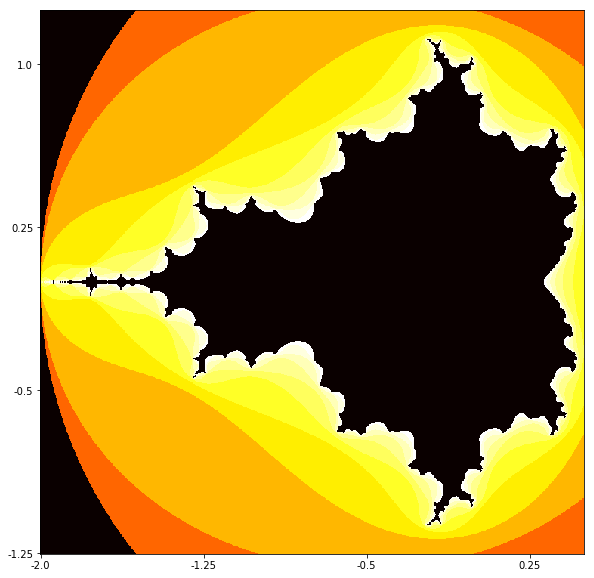
\includegraphics[width=0.9\linewidth]{Mandelbrot_d_10.png}
  \caption{Using 10 Iterates}
\end{subfigure}%
\begin{subfigure}{.33\textwidth}
  \centering
  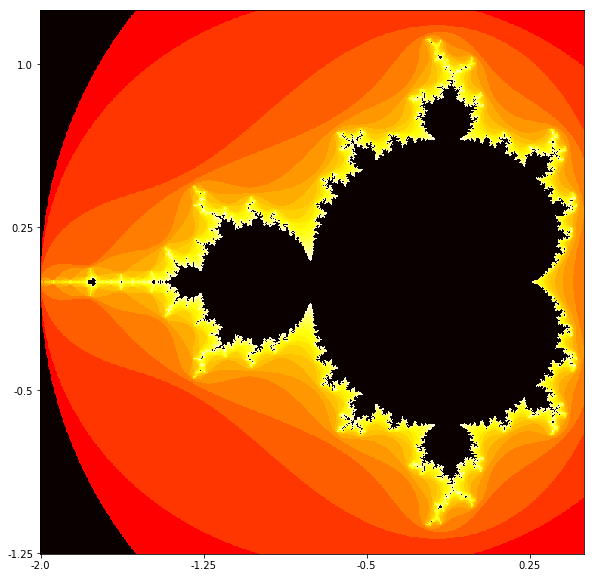
\includegraphics[width=0.9\linewidth]{Mandelbrot_d_30.png}
  \caption{Using 30 Iterates}
\end{subfigure}
\begin{subfigure}{.33\textwidth}
  \centering
  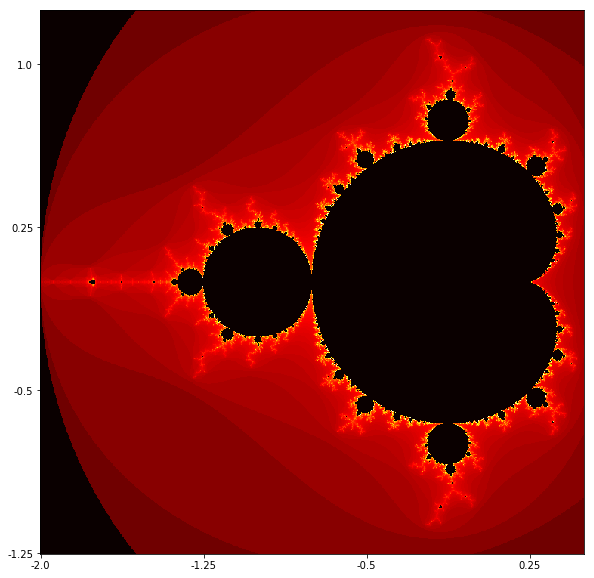
\includegraphics[width=0.9\linewidth]{Mandelbrot_d_500.png}
  \caption{Using 500 Iterates}
\end{subfigure}
\caption{Na\"ive attempts to visualize the Mandelbrot set can be deceiving.}
\label{fig:MandelbrotDIter}
\end{figure}


The second algorithm relies on a continuous estimate of iterate count \cite{Garcia2009} used in computing the Mandelbrot set. The main difference being instead of the returning the integer iteration count $n$, we return
\begin{equation}\label{contest}
\eta= n+\frac{\log\log b-\log \log \abs{z_n}}{\log 2} \text{ where $b$ is the bailout radius}
\end{equation}
which gives us continuous values for our escape iterate! This equation is actually heavily related to potential theory as will see below.\\

In order to see the origin of (\ref{contest}), we will need the following theorem (originally by B\"ottcher in 1904).
\begin{thm}\cite[Theorem 9.1]{milnor2011}\label{Butch}
  Given a monic polynomial $f$ of degree $n$, there exists a biholomorphic map $\phi$ which fixes 0 and conjugates $f$ and $z^n$.
\end{thm}

Considering again the case of $c=0$, we recall that the filled Julia set of $f$ is given by the closed unit disk $\overline{\mathbb{D}}$. On the Fatou component containing $\infty$, $\bbCS\setminus \overline{\mathbb{D}}$, we can define the \emph{potential function} of $f_0$ as
\begin{equation}
  \psi(z)=\lim\limits_{n\to\infty}\frac{\log \abs{z^n}}{2^n}.
\end{equation}
Using the theorem of B\"ottcher, we can conjugate the dynamics of $z^2+c$ to $z^2$ on the complements of their respective filled Julia sets.
\begin{thm}[B\"ottcher Coordinates]
  There exists a biholomorphic map $\phi$ such that $f_c$ is conjugate to $f_0$ in a neighborhood of infinity.
\end{thm}
\begin{rem}
  In fact, for $c\in \Mand$, our conjugacy $\phi$ can be extended to the domains $\bbCS\setminus \overline{\mathbb{D}}$ and $\bbCS\setminus K(f_c)$. This extension can be used to give another proof that the Mandelbrot set is connected.
\end{rem}
\begin{proof}
Making the substitutions $w=\frac{1}{z}$ and $g(w)=\frac{1}{f(1/w)}$, we can conjugate the point $\infty$ to 0. Using \cref{Butch}, we can get a conjugacy between $w^2$ and $g(w)$ near zero. This corresponds to a conjugacy between $z^2$ and $f_c$ near $\infty$.
\end{proof}

Using that $\abs{\phi (f_c^n (z))}=\abs{\phi(z)}^{2n}$ for any large enough $n$, the existence of this conjugacy $\phi$ tells us that our potential function $\psi$ is the same for every $f_c$ though on a different domain. Therefore, for some large $b$, if we take the first iterate $n$ such that $f_c^n(0)>b$, then we can find some real number $\eta$ such that
\begin{equation}
  \frac{\log \abs{f_c^n(0)}}{2^n}=\frac{\log b}{2^{\eta}}.
\end{equation}
Rearranging the above equation and solving for $\eta$ gives us the estimate used in (\ref{contest}).

The caveat of this method is that we must pick much larger bailout radius $b$, so that $z^2+c$ can begin to resemble $z^2$ `near infinity' in the sense of B\"ottcher allowing us to use our estimate.
The modification of the code to include the estimate given by (\ref{contest}) can be seen in the following snippet:

\inputminted[mathescape]{python}{code-snippets/Mandelbrot_c.py}

\begin{figure}[h]
  \centering
  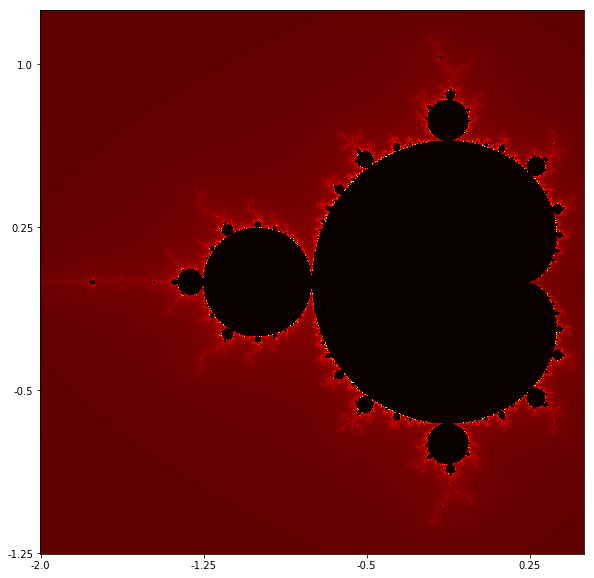
\includegraphics[width=0.45\textwidth]{Mandelbrot_c_5000.png}
  \caption{Mandelbrot Set Using Normalized Iteration Count}
\end{figure}

This Normalized Iteration Count algorithm produces a much `smoother' image and allows us to see many more details of the Mandelbrot set. In particular, points for which escape takes a large number of iterates are highlighted as a lighter color and are often close to $\Mand$ itself. This feature of our continuous estimate allows us to visualize finer details of the Mandelbrot set and enables us to zoom in more confidently, though we may need to increase the maximum number of iterates to faithfully depict those $c$ for which the orbit of 0 escapes slowly under $f_c$. This added clarity does not come at much cost, with this algorithm taking $383 \pm 5.69$ milliseconds per loop to execute on average.\\

Zooming allows us to see some of the (quasi-)self-similarity that $\Mand$ displays, characteristic of its fractal nature. In \cref{fig:MandelbrotZoom}, we see that zooming in on the small island near $c=-1.457$ reveals a pattern resembling the larger set $\Mand$. This self-similarity is not limited to the appearance of mini Mandelbrot sets, but we can actually see similarities to the Julia sets of a given polynomial $z^2+c$ and the neighborhood of $c$ near the Mandelbrot set.\\

\begin{figure}[h]
\centering
\begin{subfigure}{.4\textwidth}
  \centering
  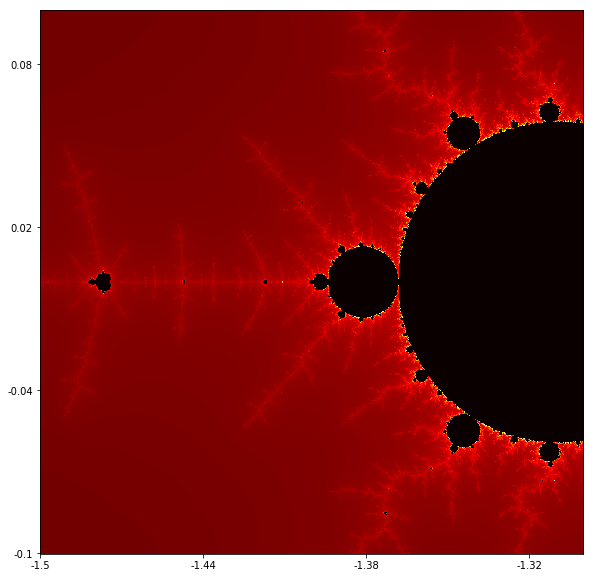
\includegraphics[width=.8\linewidth]{Mandelbrot_c_zoom.png}
  \caption{Zooming onto left side.}
\end{subfigure}%
\begin{subfigure}{.4\textwidth}
  \centering
  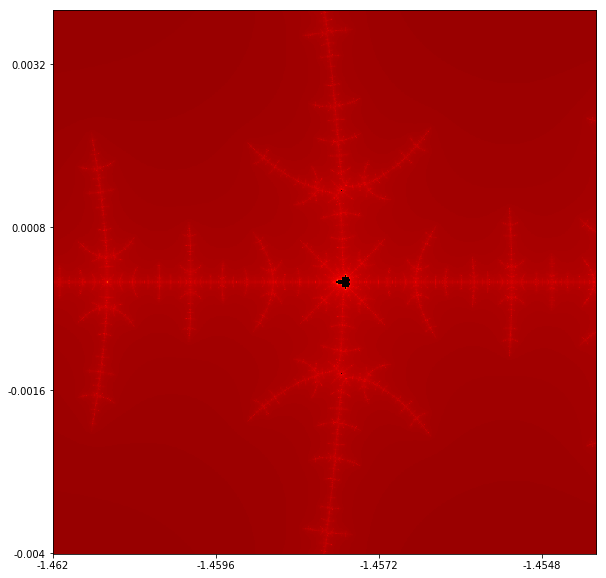
\includegraphics[width=.8\linewidth]{Mandelbrot_c_zoom1.png}
  \caption{Zooming into island in middle.}
\end{subfigure}
\begin{subfigure}{.4\textwidth}
  \centering
  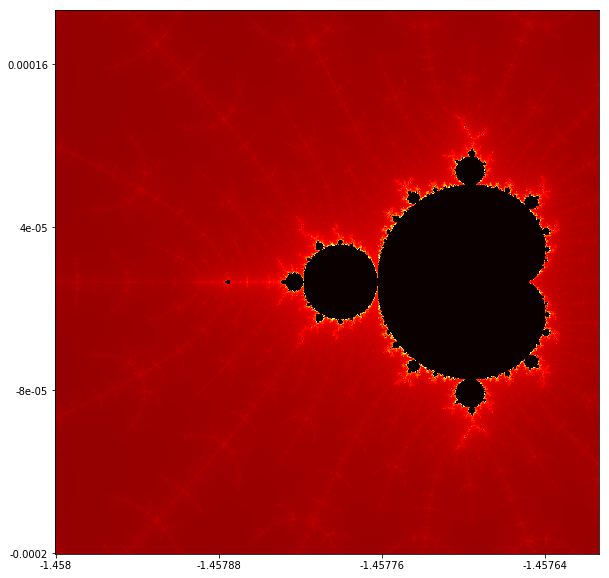
\includegraphics[width=.8\linewidth]{Mandelbrot_c_zoom2.png}
  \caption{Zooming reveals a mini $\Mand$!}
\end{subfigure}
\caption{The Normalized Iteration Count algorithm allows us the clarity needed to view finer features of the Mandelbrot set.}
\label{fig:MandelbrotZoom}
\end{figure}

Another relationship between the Mandelbrot set and the Julia set is that for any parameter $c\in\Mand$ corresponds to $f_c$  having a connected Julia set $J(f_c)$ i.e. $\Mand$ is the connectivity locus for the family $f_c$. Similarly, when $c\notin\Mand$, the the Julia set $J(f_c)$ is a Cantor set. Though we will not prove these statements one can see examples of this phenomenon using the various code snippets and figures above. These observations have proved to be helpful in efforts to approach the following open question.

\begin{conj}[MLC Conjecture]
  The Mandelbrot set $\Mand$ is locally connected.
\end{conj}

The work of Jean-Christophe Yoccoz towards this conjecture, proving that the Mandelbrot set is locally connected at finitely renormalizable $c\in \Mand$, helps to reveal a more general relation between the Mandelbrot and Julia sets. By understanding the dynamical properties of $f_c$ via its Julia set (establishing local connectivity of $J(f_c)$) one can move to parameter space  $\Mand$ studying the properties of the Mandelbrot set itself (local connectivity at $c$).\\

We can see an application of this idea in the proof of the following theorem.
\begin{thm}
  The Mandelbrot set $\Mand$ is compact and simply connected.
\end{thm}
\begin{proof}
By \cref{Mescape}, $\Mand$ is precisely the set $\{c\mid \abs{f_c^n(0)}\leq 2\text{ for all } n\geq 0 \}$. We can then decompose $\Mand$ into intersection of the sets $\Mand_n=\{c\in\bbC \mid \abs{f^n_c(0)}\leq 2\}$. Taking any sequence of parameters $(c_i)_{i=1}^\infty$ in $\Mand_n$, we see that  $\abs{f^n_{c_i}(0)}$ must converge to $\abs{f^n_c(0)}$ since $f_c$ is continuous in $c$. Since the sequence $\abs{f^n_{c_i}(0)}$ is bounded by 2, $\abs{f^n_c(0)}\leq 2$. Therefore, each $\Mand_n$ is closed, and likewise $\Mand=\bigcap_{n=1}^\infty \Mand_n$ must be closed. The Mandelbrot set $\Mand$ is additionally compact since it is contained in the circle of radius 2 centered at the origin and thereby bounded. \\

The proof of the second statement follows theorem 8.6.1 of \cite{brin_stuck_2002}. Suppose that $\bbC\setminus\Mand$ contains some bounded, connected component $A$. Since $A\subset\bbC\setminus\Mand$, we can there is some $n$ such that \[
\sup_{c\in\overline{A}}f^n_c(0)>2.
\]
Therefore, by the maximum modulus principle, there must be some parameter $\gamma$ on the boundary of $A$ such that $f^n_\gamma(0)>2$. Since the boundary of $A$ must be contained in  $\Mand$ because it is closed, this gives a contradiction. Therefore, there cannot be any bounded component of $\bbC\setminus \Mand$, so $\bbC\setminus \Mand$ consists of one unbounded connected component containing $\infty$ and is connected itself. Therefore, its complement $\Mand$ must be simply connected.
\end{proof}

With these tools and properties in mind, we're now in good shape to try and tackle the case of higher degree polynomials.


%\begin{itemize}
%  \item Talk about the interest in visualizing the Mandelbrot set. (This work can be deceptive due to the precision of machines. At first glance, the Mandelbrot set appears to not be connected but Douady and Hubbard prove it is connected. Better visualization methods can help make this more apparent.)

%  \item Switch to discussion to continuous algorithm, relate to Böttcher theorem, conjugating $z^2+c$ to $z^2$ in a neighborhood of $\infty$ (one of your sources has formula and proof of the formula! in case $d=2$).
%  \item Highlight interplay with the `Mandelbrot set' (bifrucation plot) along the real line!

%\end{itemize}


  \subsection{Higher Degree Polynomials \& the Shift Locus}
We might try to generalize the methods in the previous section to compute one complex-dimensional slices of the shift locus.

\begin{defn}\cite{demarco2011}
Let $\Poly_d$ denote the space of monic degree $d$ polynomials. We define the \emph{shift locus in dimension $d$} to be
\begin{equation}
  \Shift{d}=\{f\in \Poly_d \mid \abs{f^n(z_\ast)}\to\infty \text{ for every $z_\ast\in\bbC$ such that $f'(z_\ast)=0$} \}.
\end{equation}
\end{defn}
The first thing to notice is that if we identify $\Poly_2$ with $\bbC$ via $c\leftrightarrow z^2+c$, then we see that $\Mand=\bbC\setminus \Shift{2}$ since 0 is the only critical points of $z^2+c$. From this, we see that the Mandelbrot set is the complement of the shift locus in two dimensions. Keeping this in mind, our next question may be about how our methods in computing and understand the Mandelbrot set might generalize. In $d$ dimensions, just finding the critical points of a given polynomial requires computing the roots of a $(d-1)$ degree polynomial. In higher dimensions, solving this equation and finding these critical points and checking the boundedness of its orbits becomes increasingly difficult from a computational standpoint. Luckily, in the case of $d=3$, the problem is still easily tractable due to the quadratic formula.\\

\begin{figure}[h]
\centering
\begin{subfigure}{.32\textwidth}
  \centering
  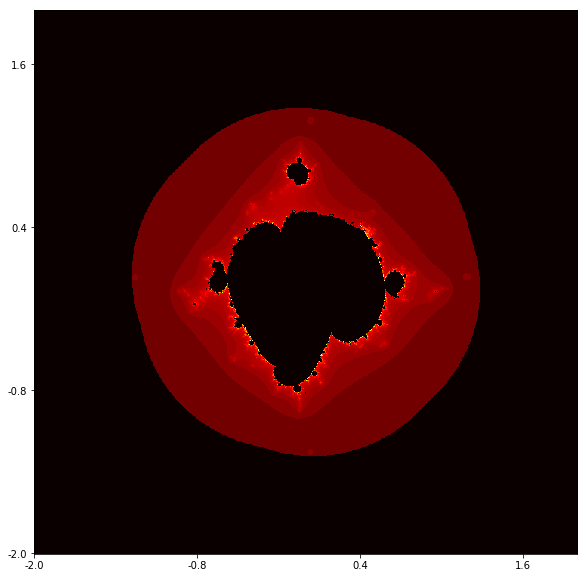
\includegraphics[width=.7\linewidth]{ShiftLocus3b1.png}
  \caption{$b=-0.2+0.2i$}
\end{subfigure}%
\begin{subfigure}{.32\textwidth}
  \centering
  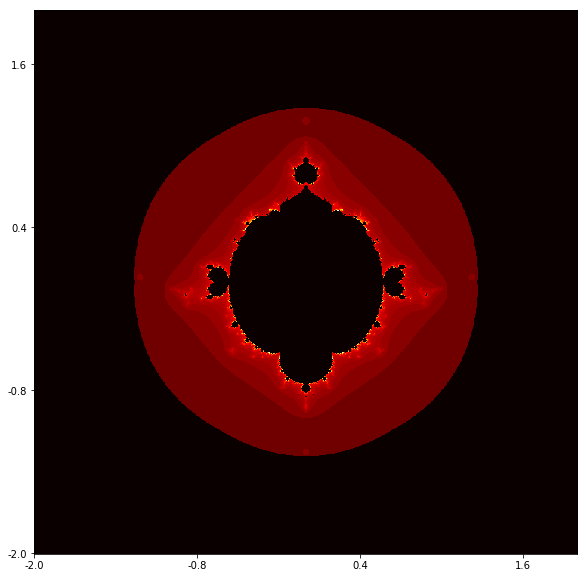
\includegraphics[width=.7\linewidth]{ShiftLocus3b2.png}
  \caption{$b=0.2i$}
\end{subfigure}
\begin{subfigure}{.32\textwidth}
  \centering
  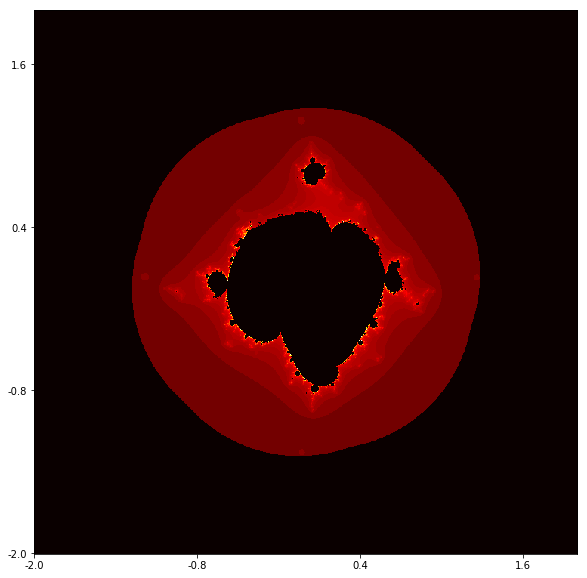
\includegraphics[width=.7\linewidth]{ShiftLocus3b3.png}
  \caption{$b=0.2+0.2i$}
\end{subfigure}
\begin{subfigure}{.32\textwidth}
  \centering
  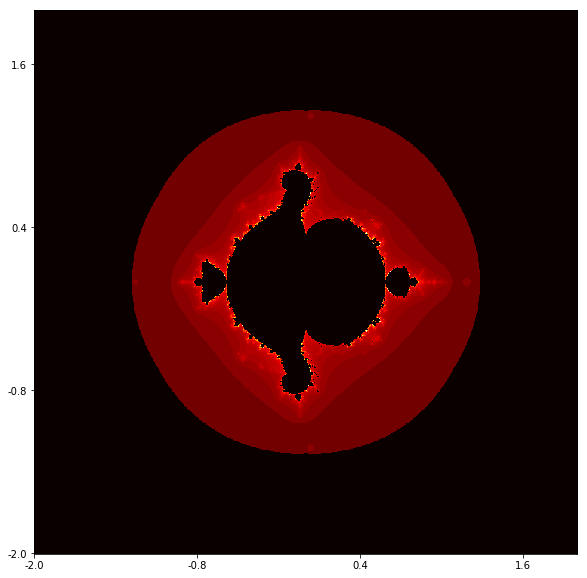
\includegraphics[width=.7\linewidth]{ShiftLocus3b4.png}
  \caption{$b=-0.2$}
\end{subfigure}
\begin{subfigure}{.32\textwidth}
  \centering
  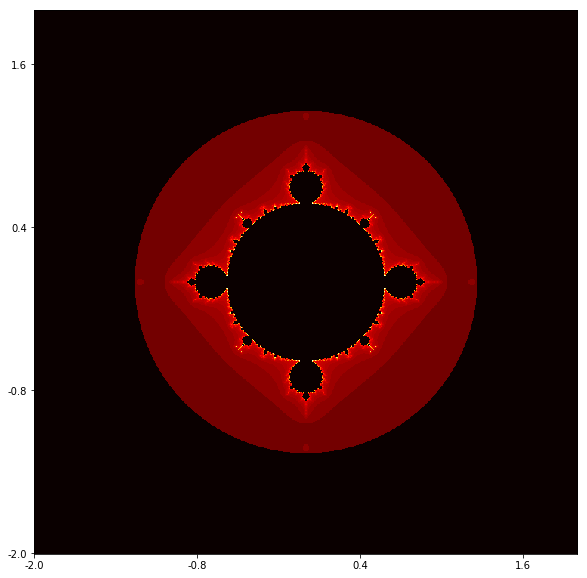
\includegraphics[width=.7\linewidth]{ShiftLocus3b5.png}
  \caption{$b=0$}
\end{subfigure}%
\begin{subfigure}{.32\textwidth}
  \centering
  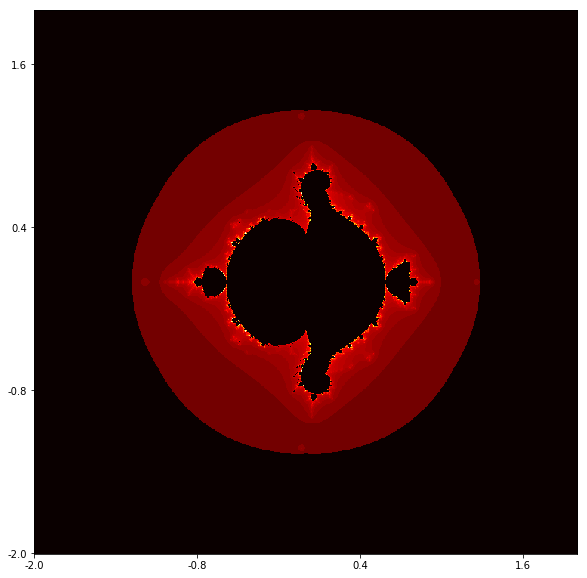
\includegraphics[width=.7\linewidth]{ShiftLocus3b6.png}
  \caption{$b=0.2$}
\end{subfigure}
\begin{subfigure}{.32\textwidth}
  \centering
  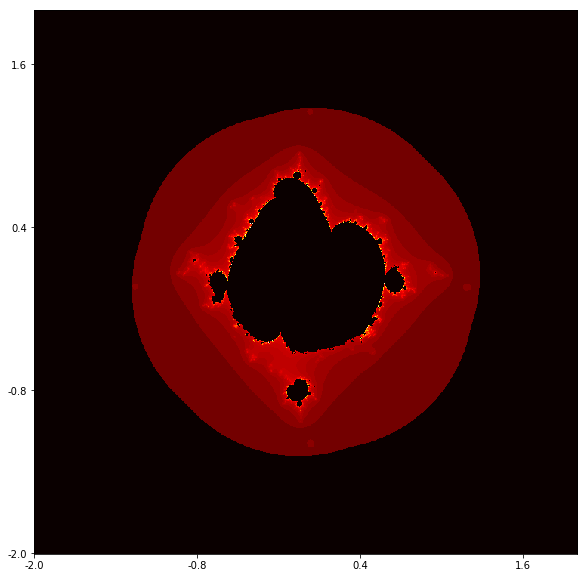
\includegraphics[width=.7\linewidth]{ShiftLocus3b7.png}
  \caption{$b=-0.2-0.2i$}
\end{subfigure}
\begin{subfigure}{.32\textwidth}
  \centering
  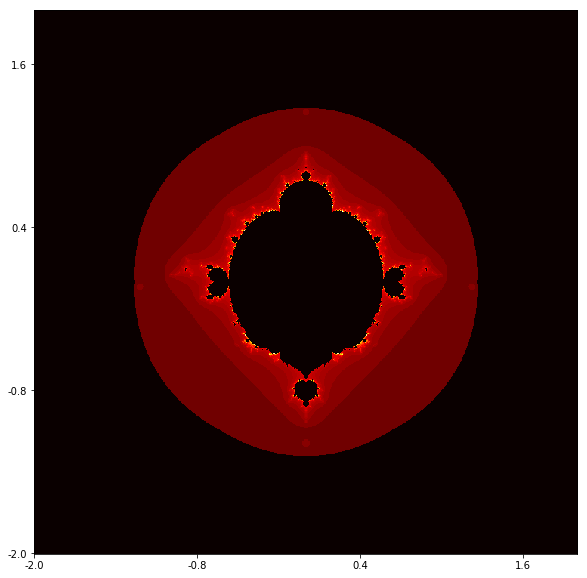
\includegraphics[width=.7\linewidth]{ShiftLocus3b8.png}
  \caption{$b=-0.2$}
\end{subfigure}
\begin{subfigure}{.32\textwidth}
  \centering
  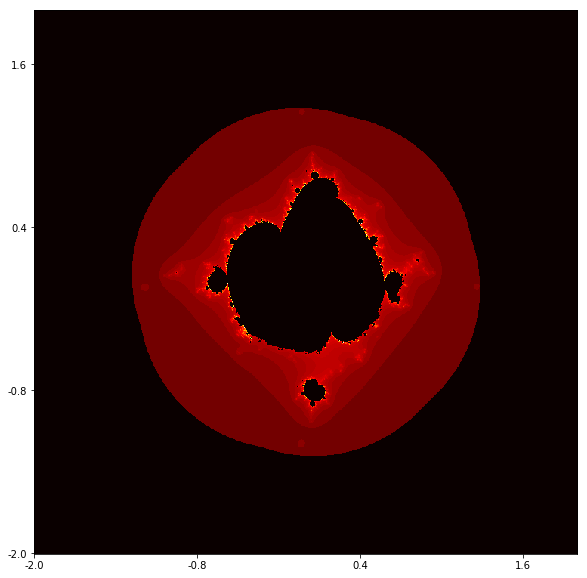
\includegraphics[width=.7\linewidth]{ShiftLocus3b9.png}
  \caption{$b=-0.2+0.2i$}
\end{subfigure}
\caption{$a$-Parameter Space using $z\mapsto z^3-a^2z+b$}
\label{fig:ShiftLocusB}
\end{figure}

In what follows, we're going to restrict to the normal family of degree 3 polynomials given by $f_{a,b}(z)=z^3-3a^2z+b$. We can identify this space with $\bbC^2$ and use this to generate one complex-dimensional slices of $\Shift{3}$. Iterating this family of polynomials at its critical points $\pm a$ can be done with the following code:\\

\inputminted[mathescape]{python}{code-snippets/ShiftLocus3.py}

This code allows us to produce slices of $\Shift{3}$ in either the $a$ parameter space for a fixed $b$ or in $b$ parameter space for a fixed $a$ by finding points which are in the complement of the shift locus $\Shift{3}$. Either or is easily implemented similarly to the Mandelbrot or Julia set code presented early. Using this algorithm, we can produces images like those of \cref{fig:ShiftLocusA} and \cref{fig:ShiftLocusB}. In a way, this is the most na\"ive way of computing the shift locus, borrowing heavily from our discrete escape iterate count algorithm for computing the Mandelbrot set. The na\"ivety is reflected in the execution time with it taking 2.88 seconds $\pm$ 158 milliseconds to generate a slice of the $a$-parameter space, and 4.73 seconds $\pm$ 116 milliseconds for $b$-parameter space on average.

\begin{figure}[h]
\centering
\begin{subfigure}{.32\textwidth}
  \centering
  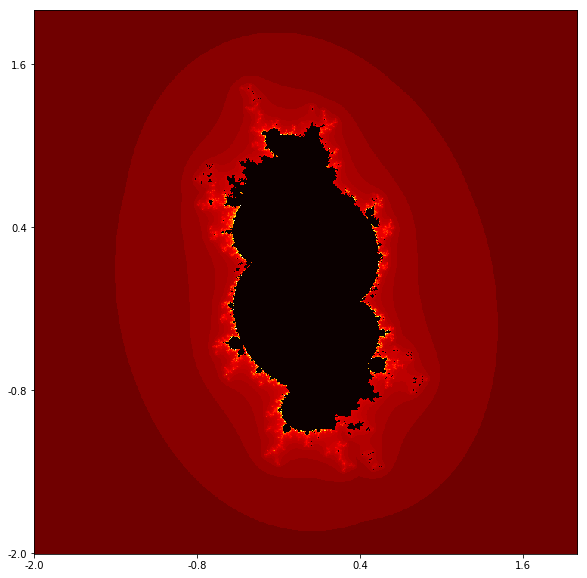
\includegraphics[width=0.7\linewidth]{ShiftLocus3a1.png}
  \caption{$a=-0.2+0.2i$}
\end{subfigure}%
\begin{subfigure}{.32\textwidth}
  \centering
  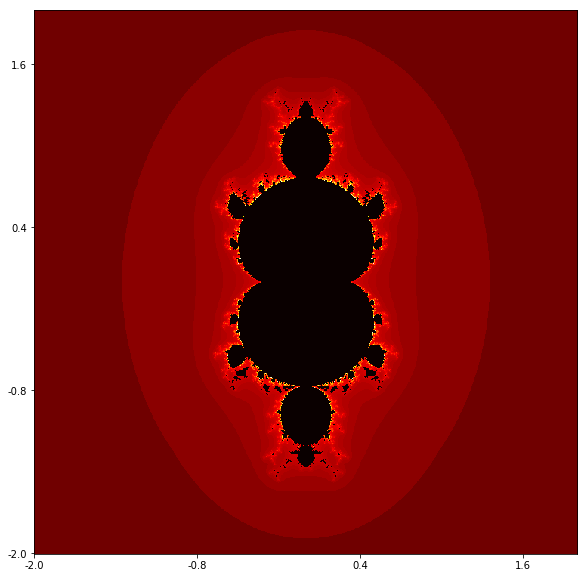
\includegraphics[width=0.7\linewidth]{ShiftLocus3a2.png}
  \caption{$a=0.2i$}
\end{subfigure}
\begin{subfigure}{.32\textwidth}
  \centering
  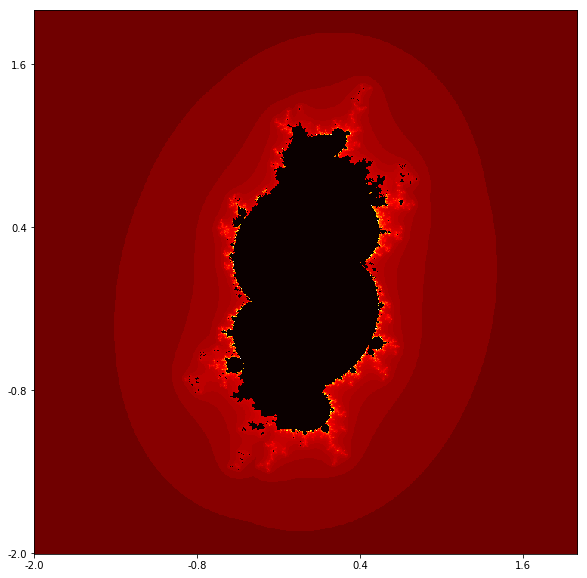
\includegraphics[width=0.7\linewidth]{ShiftLocus3a3.png}
  \caption{$a=0.2+0.2i$}
\end{subfigure}
\begin{subfigure}{.32\textwidth}
  \centering
  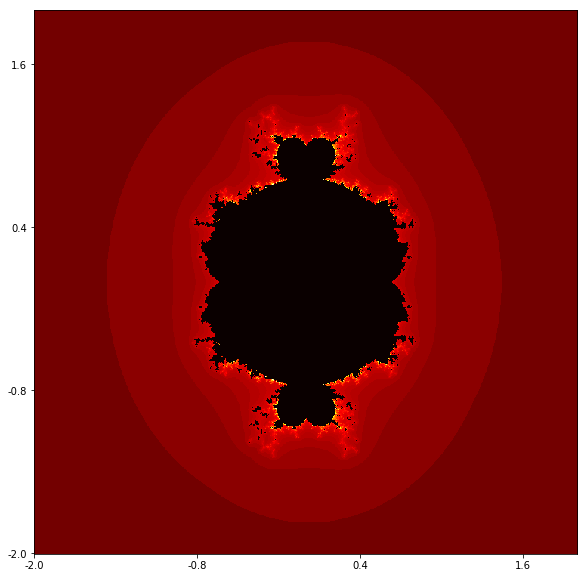
\includegraphics[width=0.7\linewidth]{ShiftLocus3a4.png}
  \caption{$a=-0.2$}
\end{subfigure}
\begin{subfigure}{.32\textwidth}\label{fig:ShiftLocus3a5}
  \centering
  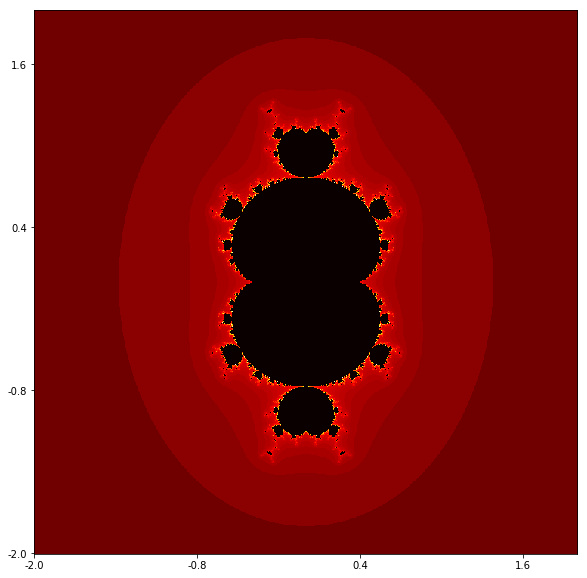
\includegraphics[width=0.7\linewidth]{ShiftLocus3a5.png}
  \caption{$a=0$}
\end{subfigure}%
\begin{subfigure}{.32\textwidth}
  \centering
  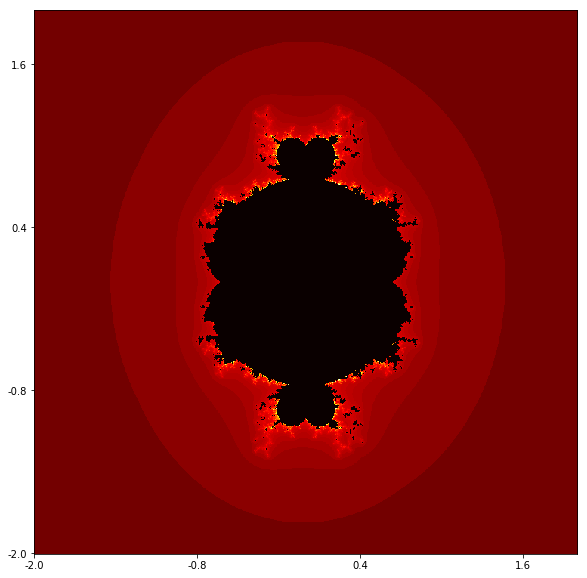
\includegraphics[width=0.7\linewidth]{ShiftLocus3a6.png}
  \caption{$a=0.2$}
\end{subfigure}
\begin{subfigure}{.32\textwidth}
  \centering
  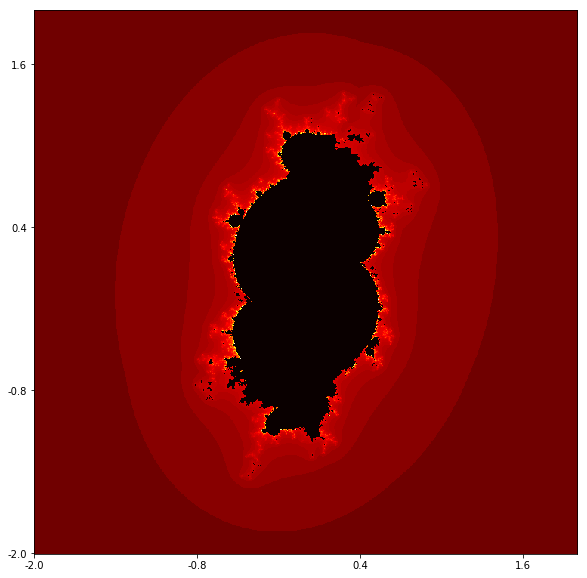
\includegraphics[width=0.7\linewidth]{ShiftLocus3a7.png}
  \caption{$a=-0.2-0.2i$}
\end{subfigure}
\begin{subfigure}{.32\textwidth}
  \centering
  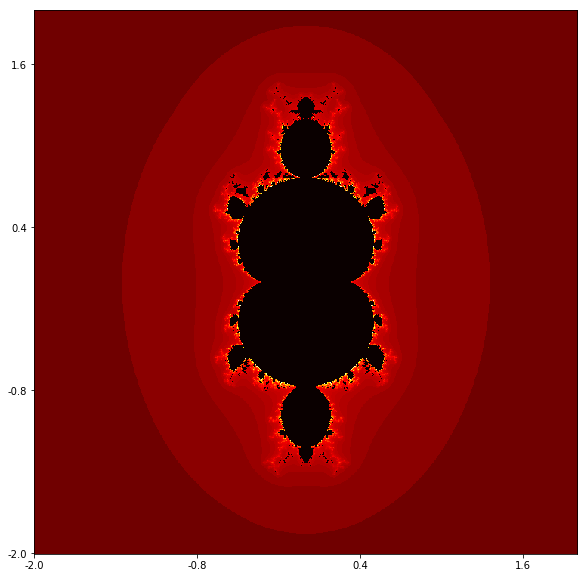
\includegraphics[width=0.7\linewidth]{ShiftLocus3a8.png}
  \caption{$a=-0.2$}
\end{subfigure}
\begin{subfigure}{.32\textwidth}
  \centering
  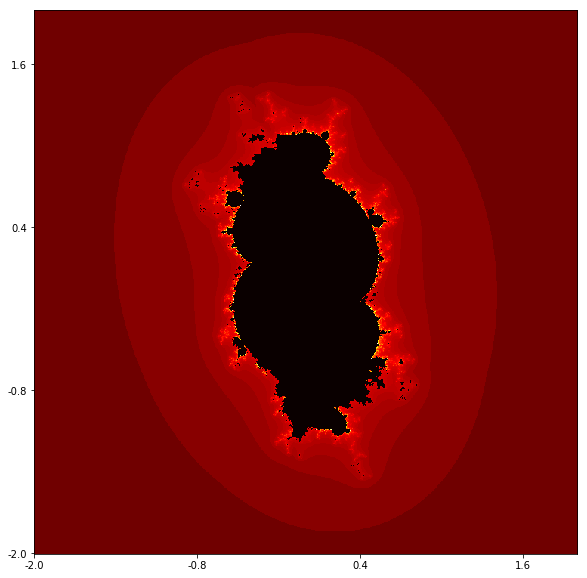
\includegraphics[width=0.7\linewidth]{ShiftLocus3a9.png}
  \caption{$a=-0.2+0.2i$}
\end{subfigure}
\caption{$b$-Parameter Space using $z\mapsto z^3-a^2z+b$}
\label{fig:ShiftLocusA}
\end{figure}



In attempting to generalize this code to higher dimensions, calculating the critical points becomes an increasingly demanding computationally.

 One might ask whether there is a similar relationship between the Julia sets of the family $z^3-a^2z+b$ and $\bbC^2\setminus\Shift{3}$, similar to one between $z^2+c$ and $\Mand$. We can make simple modifications to the julia code we presented in \cref{JuliaComp} to adjust it to the family of functions above:

 \inputminted[mathescape]{python}{code-snippets/Julia3.py}

 For reference, this algorithm takes $154 \pm 2.12$ milliseconds on average to execute. Using this updated julia function to compute the Julia sets for the above family may help provide some preliminary visual intuition for the relationship between the complement of the shift locus and the Julia set before attempting to investigate the possibility of such similarities using more advanced methods, may they be computational or otherwise mathematical in nature.

 \begin{figure}[h]
 \centering
 \begin{subfigure}{.34\textwidth}
   \centering
   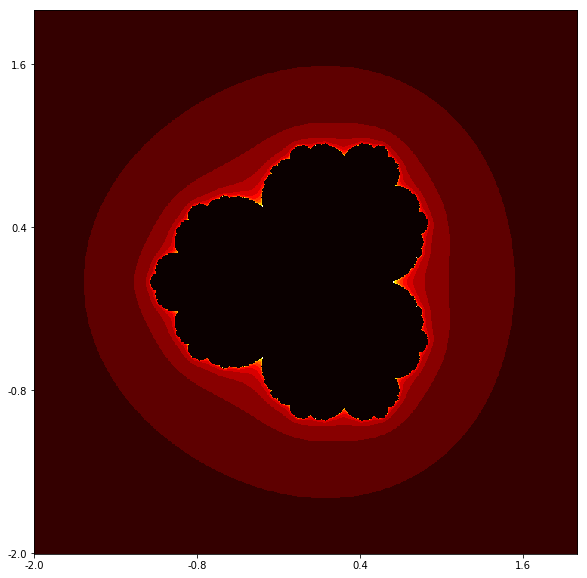
\includegraphics[width=.8\linewidth]{Julia33.png}
   \caption{b=0.38}
 \end{subfigure}%
 \begin{subfigure}{.34\textwidth}
   \centering
   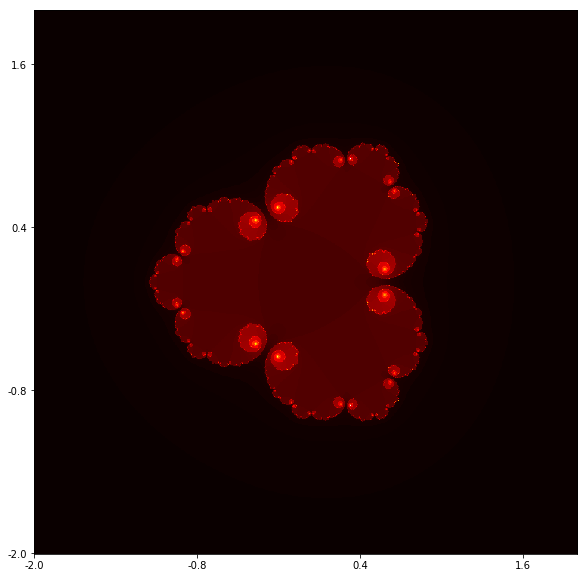
\includegraphics[width=.8\linewidth]{Julia34.png}
   \caption{b=0.4}
 \end{subfigure}
 \begin{subfigure}{.34\textwidth}
   \centering
   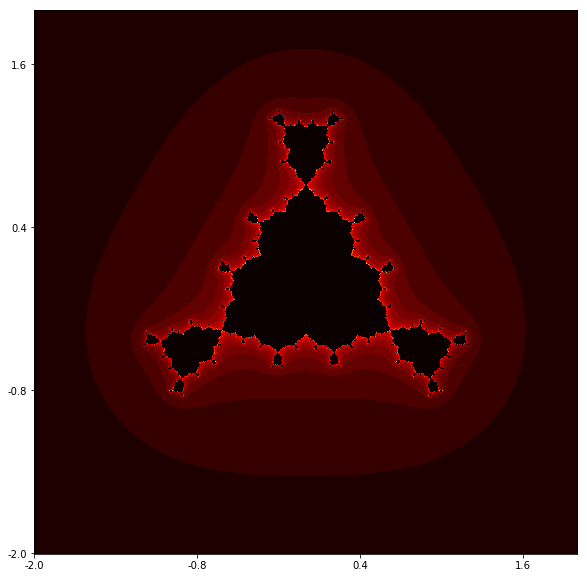
\includegraphics[width=.8\linewidth]{Julia36.png}
   \caption{b=1.08i}
 \end{subfigure}
 \begin{subfigure}{.34\textwidth}
   \centering
   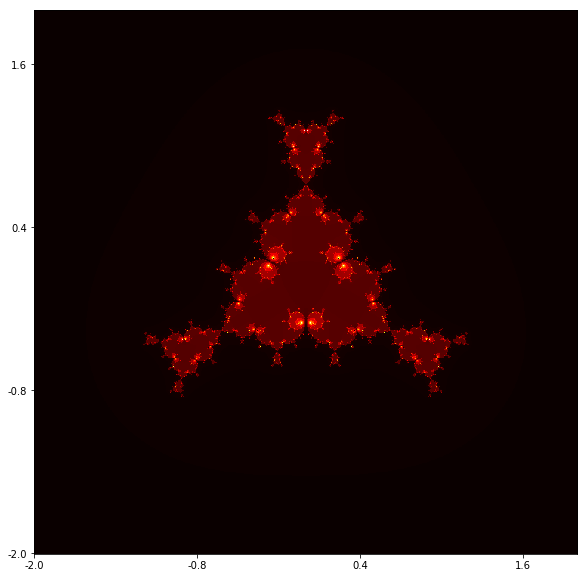
\includegraphics[width=.8\linewidth]{Julia35.png}
   \caption{b=1.09i}
 \end{subfigure}
 \caption{Julia Sets for $f_{0,b}$ near the boundary of $\Shift{3}$.}
 \label{fig:Julia3}
 \end{figure}

 With this idea in mind, we may recall that the Mandelbrot set $\bbC\setminus\Shift{2}$ is the locus of connectivity for the family of polynomials $z^2+c$. Partially motivated by the results of our computations in \cref{fig:ShiftLocusA} and \cref{fig:Julia3}, we end on the following question.

 \begin{quest}
     For which pairs of parameters $(a,b)\in\bbC^2$ are the Julia sets $J(f_{a,b})$ connected.
 \end{quest}

 Influenced by our earlier computational methods and the accompanying images, our intuition tells us that this set may be the complement of the shift locus $\bbC^2\setminus\Shift{3}$ though proving this would require additional analysis. In this way, we see that computation can help to provide visual and numerical aid in understanding mathematical problems, especially so in the case of complex dynamics.

%%% End paragraph about computation
\begin{bibdiv}

\begin{biblist}

  %\bib{ahlfors1979}{book}{
  %  title={Complex analysis: an introduction to the theory of analytic functions of one complex variable},
  %  author={Ahlfors, L.V.},
  %  isbn={9780070006577},
  %  lccn={78017078},
  %  series={International series in pure and applied mathematics},
  %  url={https://books.google.com/books?id=2MRuus-5GGoC},
  %  year={1979},
  %  publisher={McGraw-Hill}
  %}

  \bib{beardon2000}{book}{
    title={Iteration of Rational Functions: Complex Analytic Dynamical Systems},
    author={Beardon, A.F.},
    isbn={9780387951515},
    series={Graduate Texts in Mathematics},
    year={2000},
    publisher={Springer New York}
  }

  \bib{brin_stuck_2002}{book}{
   place={Cambridge},
    title={Introduction to Dynamical Systems},
    DOI={10.1017/CBO9780511755316},
    publisher={Cambridge University Press}, author={Brin, Michael},
      author={ Stuck, Garrett},
    year={2002}
  }

  \bib{demarco2011}{article}{
  	title={Combinatorics and topology of the shift locus},
  	author={De Marco, Laura},
  	year={2011}
  }

\bib{Garcia2009}{article}{
title={Coloring Dynamical Systems in the Complex Plane}
author={Garcia, Francisco}
author={Fernandez, Angel}
author={Barrallo, Javier}
author={Martin, Luis}
year={2009}

}




%\bib{geyer2016}{article}{
%	title={M 597 lecture notes topics in mathematics complex dynamics},
%	author={Geyer, L.},
%	year={2016}
%}

\bib{milnor2011}{book}{
  title={Dynamics in One Complex Variable. (AM-160): (AM-160) - Third Edition},
  author={Milnor, John},
  isbn={9781400835539},
  lccn={2005051060},
  series={Annals of Mathematics Studies},
  year={2011},
  publisher={Princeton University Press}
}

\bib{sullivan1985quasiconformal}{article}{
  title={Quasiconformal homeomorphisms and dynamics II: Structural stability implies hyperbolicity for Kleinian groups},
  author={Sullivan, Dennis},
  journal={Acta mathematica},
  volume={155},
  number={1},
  pages={243--260},
  year={1985},
  publisher={Springer}
}

\end{biblist}
\end{bibdiv}

\end{document}
